\documentclass[11pt]{article}

\author{wilricknl}
\title{3D Math Primer - Solutions chapter 2}

\usepackage{amsmath}
\usepackage{enumerate}
\usepackage{graphicx}

\begin{document}

\maketitle

\section{Solutions chapter 2}

\subsection{Exercise 1}

\begin{enumerate}[a.]
    \item
    \begin{itemize}
        \item \textbf{a} is a two dimensional row vector.
        \item \textbf{b} is a three dimensional column vector.
        \item \textbf{c} is a four dimensional column vector.
    \end{itemize}
    \item $0 + 6 - 3 + 5 = 8$
\end{enumerate}

\subsection{Exercise 2}

\begin{enumerate}[a.]
	\item Scalar.
	\item Scalar.
	\item Vector: direction north and magnitude 2 blocks.
	\item 600 mph is scalar and altitude is also scalar.
\end{enumerate}


\subsection{Exercise 3}

\begin{enumerate}[a.]
	\item % a
$
\begin{bmatrix}
0 & 2
\end{bmatrix}
$
	\item % b
$
\begin{bmatrix}
0 & -2
\end{bmatrix}
$
	\item % c
$
\begin{bmatrix}
0.5 & 2
\end{bmatrix}
$
	\item % d
$
\begin{bmatrix}
0.5 & 2
\end{bmatrix}
$
	\item % e
$
\begin{bmatrix}
0.5 & -3
\end{bmatrix}
$
	\item % f
$
\begin{bmatrix}
-2 & 0
\end{bmatrix}
$
	\item % g
$
\begin{bmatrix}
-2 & 1
\end{bmatrix}
$
	\item % h
$
\begin{bmatrix}
2.5 & 2
\end{bmatrix}
$
	\item % i
$
\begin{bmatrix}
6 & 1
\end{bmatrix}
$
\end{enumerate}

\subsection{Exercise 4}

\begin{enumerate}[a.]
	\item False, the position doesn't matter, size (thus magnitude) does. So, once again: \textit{size matters}. :]
	\item True.
	\item False, you'll end up up in the same place regardless of order.
	\item False, it's the displacement from origin to the point.
\end{enumerate}

\subsection{Exercise 5}

\begin{enumerate}[a.]
	\item % a
$
-\begin{bmatrix}
3 & 7
\end{bmatrix}
=
\begin{bmatrix}
-3 & -7
\end{bmatrix}
$
	\item % b
$
||
\begin{bmatrix}
-12 & 5
\end{bmatrix}
|| = 
\sqrt{(-12)^2+(5)^2}=\sqrt{169}=13
$
	\item % c
$
||
\begin{bmatrix}
8 & -3 & \frac{1}{2}
\end{bmatrix}
|| = 
\sqrt{8^2+(-3)^2+\frac{1}{2}^2} =
\sqrt{64 + 9 + \frac{1}{4}} = \sqrt{73\frac{1}{4}}
$
	\item % d
$
3\begin{bmatrix}
4 & -7 & 0
\end{bmatrix}
=
\begin{bmatrix}
12 & -21 & 0
\end{bmatrix}
$
	\item % e
$
\begin{bmatrix}
4 & 5
\end{bmatrix}/2
=
\begin{bmatrix}
2 & \frac{5}{2}
\end{bmatrix}
$
\end{enumerate}

\subsection{Exercise 6}

\begin{enumerate}

	\item % a
$
\begin{bmatrix}
12 & 5
\end{bmatrix}/13
=
\begin{bmatrix}
\frac{12}{13} & \frac{5}{13}
\end{bmatrix}
$
	\item % b
$
\begin{bmatrix}
0 & 1
\end{bmatrix}
$
	\item % c
$
\begin{bmatrix}
\frac{8}{\sqrt{73\frac{1}{4}}} & \frac{-3}{\sqrt{73\frac{1}{4}}} & \frac{1}{2\sqrt{73\frac{1}{4}}}
\end{bmatrix}
$	
	\item % d
$
\frac{\begin{bmatrix}
-12 & 3 & 4
\end{bmatrix}}{\sqrt{(-12)^2+3^2+4^2}}=
\frac{\begin{bmatrix}
-12 & 3 & 4
\end{bmatrix}}{\sqrt{169}}=
\begin{bmatrix}
\frac{-12}{13} & \frac{3}{13} & \frac{4}{13}
\end{bmatrix}
$
	\item % e
	$
\frac{\begin{bmatrix}
1 & 1 & 1 & 1
\end{bmatrix}}{\sqrt{4}}=
\begin{bmatrix}
\frac{1}{2} & \frac{1}{2} & \frac{1}{2} & \frac{1}{2}
\end{bmatrix}
$
\end{enumerate}

\subsection{Exercise 7}

\begin{enumerate}
	\item % a
$
\begin{bmatrix}
7+6 & -2+6 & -3+-4
\end{bmatrix}=
\begin{bmatrix}
13 & 4 & -7
\end{bmatrix}
$
	\item % b
$
\begin{bmatrix}
2+-2 & 9+-9 & -1+1
\end{bmatrix}=
\begin{bmatrix}
0 & 0 & 0
\end{bmatrix}
$
	\item % c
$
\begin{bmatrix}
3-8 \\
10--7 \\
7-4
\end{bmatrix}=
\begin{bmatrix}
-5 \\
17 \\
3
\end{bmatrix}
$
	\item % d
$
\begin{bmatrix}
4--4 \\
5--5 \\
-11-11
\end{bmatrix}=
\begin{bmatrix}
8 \\
10 \\
-22
\end{bmatrix}
$
	\item % e
$
\begin{bmatrix}
3a \\
3b \\
3c
\end{bmatrix}+
\begin{bmatrix}
-8 \\
-40 \\
24
\end{bmatrix}=
\begin{bmatrix}
3a-8 \\
3b-40 \\
3c+24
\end{bmatrix}
$
\end{enumerate}

\subsection{Exercise 8}

\begin{enumerate}
	\item % a
$
\sqrt{(-14-10)^2+(30-6)^2}=
\sqrt{(-24)^2+(24)^2}=
\sqrt{1152}
$
	\item % b
$
13
$
	\item % c
$
\sqrt{(8-3)^2+(-7-10)^2+(4-7)^2}=
\sqrt{(5)^2+(-17)^2+(-3)^2}=
\sqrt{25+289+9}=\sqrt{323}
$
	\item % d
$
\sqrt{(0.5)^2+(-3)^2+(8)^2}=
\sqrt{\frac{1}{4}+9+64}=
\sqrt{73\frac{1}{4}}
$
	\item % e
$
\sqrt{400}=20
$
\end{enumerate}

\subsection{Exercise 9}

\begin{enumerate}
	\item % a
$
\begin{bmatrix}
2 \\
6
\end{bmatrix}\cdot{}
\begin{bmatrix}
-3 \\
8
\end{bmatrix}=
2\cdot{}-3+6\cdot{}8=-6+48=42
$
	\item % b
$
-7\begin{bmatrix}
1 \\
2
\end{bmatrix}\cdot{}
\begin{bmatrix}
11 \\
-4
\end{bmatrix}=
\begin{bmatrix}
-7 \\
-14
\end{bmatrix}\cdot{}
\begin{bmatrix}
11 \\
-4
\end{bmatrix}=-7\cdot{}11+-14\cdot{}-4=-77+56=-21
$
	\item % c
$
10+
\begin{bmatrix}
-5 \\
1 \\
3
\end{bmatrix}\cdot{}
\begin{bmatrix}
4 \\
-13 \\
9
\end{bmatrix}=
10+(-20-13+27)=37-33=4
$
	\item % d
$
3\begin{bmatrix}
-2 \\
0 \\
4
\end{bmatrix}\cdot{}
\left(
\begin{bmatrix}
8 \\
-2 \\
\frac{3}{2}
\end{bmatrix}+
\begin{bmatrix}
0 \\
9 \\
7
\end{bmatrix}
\right)=
\begin{bmatrix}
-6 \\
0 \\
12
\end{bmatrix}\cdot{}
\begin{bmatrix}
8 \\
7 \\
8\frac{1}{2}
\end{bmatrix}=
-48+85+17=54
$
\end{enumerate}

\subsection{Exercise 10}

$\textbf{v}_\|=(\hat{\textbf{n}}\cdot{}\textbf{v})\hat{\textbf{n}}=
\left(\begin{bmatrix}
\sqrt{2}/2 \\
\sqrt{2}/2 \\
0
\end{bmatrix}\cdot{}
\begin{bmatrix}
4 \\
3 \\
-1
\end{bmatrix}
\right)
\begin{bmatrix}
\sqrt{2}/2 \\
\sqrt{2}/2 \\
0
\end{bmatrix}= \\
(\frac{4\sqrt{2}}{2}+\frac{3\sqrt{2}}{2})
\begin{bmatrix}
\sqrt{2}/2 \\
\sqrt{2}/2 \\
0
\end{bmatrix}
=
\begin{bmatrix}
14/4 \\
14/4 \\
0
\end{bmatrix}$

$\textbf{v}_\bot=\textbf{v}-\textbf{v}_\|=
\begin{bmatrix}
4 \\
3 \\
-1
\end{bmatrix}-
\begin{bmatrix}
14/4 \\
14/4 \\
0
\end{bmatrix}=
\begin{bmatrix}
1/2 \\
-1/2 \\
-1
\end{bmatrix}
$

\subsection{Exercise 11}

Important to remember is that is stated that $\textbf{a}\cdot{}\textbf{b}=\|\textbf{a}\|\|\textbf{b}\|\cos\theta$, this is used in the second-last step.

$\|\textbf{a}-\textbf{b}\|^2=(\textbf{a}-\textbf{b})(\textbf{a}-\textbf{b})=\textbf{a}^2-2\textbf{a}\textbf{b}+\textbf{b}^2=\|\textbf{a}\|^2+\|\textbf{b}\|^2-2\|\textbf{a}\|\|\textbf{b}\|\cos\theta$

\subsection{Exercise 12}

The cosine difference identity is used to simplify the equation.

$\textbf{a}\cdot{}\textbf{b}=a_xb_x+a_yb_y=\|a\|\cos\theta\|b\|\cos\phi+\|a\|\sin\theta\|b\|\sin\phi=\|a\|\|b\|(\cos\theta\cos\phi+\sin\theta\sin\phi)=\|a\|\|b\|\cos(\theta-\phi)$

\subsection{Exercise 13}

\begin{enumerate}[a]
	\item %a
	\begin{enumerate}
		\item % a x b
$\textbf{a} \times \textbf{b}=
\begin{bmatrix}
0 \\
-1 \\
0
\end{bmatrix}\times
\begin{bmatrix}
0 \\
0 \\
1
\end{bmatrix}=
\begin{bmatrix}
-1 \\
0 \\
0
\end{bmatrix}$
		\item % b x a
$\textbf{b} \times \textbf{a}=-(\textbf{a} \times \textbf{b})=
-\begin{bmatrix}
-1 \\
0 \\
0
\end{bmatrix}=
\begin{bmatrix}
1 \\
0 \\
0
\end{bmatrix}$
	\end{enumerate}
	\item %b
	\begin{enumerate}
		\item % a x b
$\textbf{a} \times \textbf{b}=
\begin{bmatrix}
-2 \\
4 \\
1
\end{bmatrix}\times
\begin{bmatrix}
1 \\
-2 \\
-1
\end{bmatrix}=
\begin{bmatrix}
-4--2 \\
1-2 \\
4-4
\end{bmatrix}=
\begin{bmatrix}
-2 \\
-1 \\
0
\end{bmatrix}$
		\item % b x a
$\textbf{b} \times \textbf{a}=-(\textbf{a} \times \textbf{b})=
-\begin{bmatrix}
-2 \\
-1 \\
0
\end{bmatrix}=
\begin{bmatrix}
2 \\
1 \\
0
\end{bmatrix}$
	\end{enumerate}
	\item %c
	\begin{enumerate}
		\item % a x b
$\textbf{a} \times \textbf{b}=
\begin{bmatrix}
3 \\
10 \\
7
\end{bmatrix}\times
\begin{bmatrix}
8 \\
-7 \\
4
\end{bmatrix}=
\begin{bmatrix}
40--49 \\
56-12 \\
-21-80
\end{bmatrix}=
\begin{bmatrix}
89 \\
44 \\
-101
\end{bmatrix}$
		\item % b x a
$\textbf{b} \times \textbf{a}=-(\textbf{a} \times \textbf{b})=
-\begin{bmatrix}
89 \\
44 \\
-101
\end{bmatrix}=
\begin{bmatrix}
-89 \\
-44 \\
101
\end{bmatrix}$
	\end{enumerate}
\end{enumerate}

\subsection{Exercise 14}

$$
\begin{array}{cc}
\textbf{a}=
\begin{bmatrix}
a_x \\
a_y \\
a_z
\end{bmatrix}, &
\textbf{b}=
\begin{bmatrix}
b_x \\
b_y \\
b_z
\end{bmatrix}
\end{array}
$$

$$\|\textbf{a} \times \textbf{b}\|=$$
$$\sqrt{(a_yb_z-a_zb_y)^2+(a_zb_x-a_xb_z)^2+(a_xb_y-a_yb_x)^2}=$$
$$
\sqrt{
\begin{split}
(a_yb_z)^2-2a_ya_zb_yb_z+(a_zb_y)^2 + \\
(a_zb_x)^2-2a_xa_zb_xb_z+(a_xb_z)^2 + \\
(a_xb_y)^2-2a_ya_zb_xb_y+(a_yb_x)^2
\end{split}
}=
$$
$$\cdots{}$$
$$\sqrt{(a_x^2+a_y^2+a_z^2)(b_x^2+b_y^2+b_z^2)-(a_xb_x+a_yb_y+a_zb_z)^2}=$$
$$\sqrt{\|\textbf{a}\|^2\|\textbf{b}\|^2-\left(\textbf{a}\cdot{}\textbf{b}\right)^2}=$$
$$\sqrt{\|\textbf{a}\|^2\|\textbf{b}\|^2\left(1-\left(\frac{\textbf{a}\cdot{}\textbf{b}}{\|\textbf{a}\|\|\textbf{b}\|}\right)^2\right)}=$$
$$\sqrt{\|\textbf{a}\|^2}\sqrt{\|\textbf{b}\|^2}\sqrt{1-\left(\frac{\textbf{a}\cdot{}\textbf{b}}{\|\textbf{a}\|\|\textbf{b}\|}\right)^2}=$$
$$\|\textbf{a}\|\|\textbf{b}\|\sqrt{1-\left(\frac{\textbf{a}\cdot{}\textbf{b}}{\|\textbf{a}\|\|\textbf{b}\|}\right)^2}=$$
$$\|\textbf{a}\|\|\textbf{b}\|\sqrt{1-\cos\theta^2}=$$
$$\|\textbf{a}\|\|\textbf{b}\|\sin\theta$$

\subsection{Exercise 15}

\begin{enumerate}[a.]
	\item % a
\begin{enumerate}
	\item % a
$$
\begin{array}{l}
\|
\begin{bmatrix}
3 & 4
\end{bmatrix}\|_1 = |3| + |4| = 7 \\
\|
\begin{bmatrix}
3 & 4
\end{bmatrix}\|_2 = \sqrt{|3|^2+|4|^2}=5\\
\|
\begin{bmatrix}
3 & 4
\end{bmatrix}\|_3 = \sqrt[3]{|3|^3+|4|^3}=\sqrt[3]{27+64}=\sqrt[3]{91}\\
\|
\begin{bmatrix}
3 & 4
\end{bmatrix}\|_\infty = \max(|3|, |4|) = 4
\end{array}
$$
	\item % b
$$
\begin{array}{l}
\|
\begin{bmatrix}
5 & -12
\end{bmatrix}\|_1 = |5| + |-12| = 17 \\
\|
\begin{bmatrix}
5 & -12
\end{bmatrix}\|_2 = \sqrt{|5|^2+|-12|^2}=13\\
\|
\begin{bmatrix}
5 & -12
\end{bmatrix}\|_3 = \sqrt[3]{|5|^3+|-12|^3} \\
\|
\begin{bmatrix}
5 & -12
\end{bmatrix}\|_\infty = \max(|5|, |-12|) = 12
\end{array}
$$
	\item % c
$$
\begin{array}{l}
\|
\begin{bmatrix}
-2 & 10 & -7
\end{bmatrix}\|_1 = |-2| + |10| + |-7| = 19 \\
\|
\begin{bmatrix}
-2 & 10 & -7
\end{bmatrix}\|_2 = \sqrt{|-2|^2+|10|^2+|-7|^2}=\sqrt{153}\\
\|
\begin{bmatrix}
-2 & 10 & -7
\end{bmatrix}\|_3 = \sqrt[3]{|-2|^3+|10|^3+|-7|^3} \\
\|
\begin{bmatrix}
-2 & 10 & -7
\end{bmatrix}\|_\infty = \max(|-2|, |10|, |-7|) = 10
\end{array}
$$
	\item % d
$$
\begin{array}{l}
\|
\begin{bmatrix}
6 & 1 & -9
\end{bmatrix}\|_1 = |6| + |1| + |-9| = 16 \\
\|
\begin{bmatrix}
6 & 1 & -9
\end{bmatrix}\|_2 = \sqrt{|6|^2+|1|^2+|9|^2}=\sqrt{36+1+81}=\sqrt{118}\\
\|
\begin{bmatrix}
6 & 1 & -9
\end{bmatrix}\|_3 = \sqrt[3]{|6|^3+|1|^3+|-9|^3} \\
\|
\begin{bmatrix}
6 & 1 & -9
\end{bmatrix}\|_\infty = \max(|6|, |1|, |-9|) = 9
\end{array}
$$
	\item % e
$$
\begin{array}{l}
\|
\begin{bmatrix}
-2 & -2 & -2 & -2
\end{bmatrix}\|_1 = |-2| + |-2| + |-2| + |-2| = 8 \\
\|
\begin{bmatrix}
-2 & -2 & -2 & -2
\end{bmatrix}\|_2 = \sqrt{|-2|^2+|-2|^2+|-2|^2+|-2|^2}=\sqrt{16}= 4 \\
\|
\begin{bmatrix}
-2 & -2 & -2 & -2
\end{bmatrix}\|_3 = \sqrt[3]{4|-2|^3} \\
\|
\begin{bmatrix}
-2 & -2 & -2 & -2
\end{bmatrix}\|_\infty = \max(|-2|, |-2|, |-2|, |-2|) = 2
\end{array}
$$
\end{enumerate}
	\item % b
	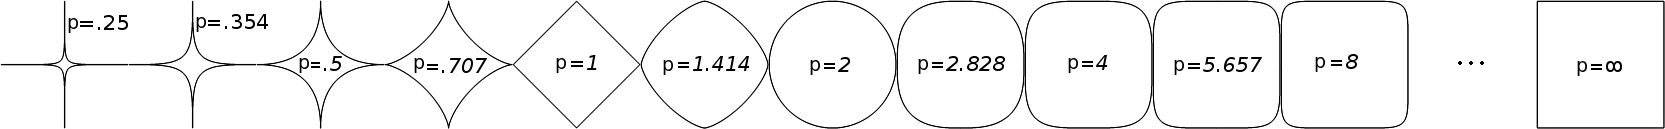
\includegraphics[width=\textwidth]{unit_circles}
\end{enumerate}

\subsection{Exercise 16}

$\sqrt{2^2+2^2+2^2}=\sqrt{12}=3.46\dots{}$, so the man can carry it diagonally.

\subsection{Exercise 17}

$\vec{\textbf{a}}+\vec{\textbf{b}}+\vec{\textbf{c}}+\vec{\textbf{d}}+\vec{\textbf{e}}+\vec{\textbf{f}}=
\begin{bmatrix}
-1 + 1 + 3 -1 - 6 - 1 \\
3 + 3 - 2 - 2 + 4 - 3
\end{bmatrix}=
\begin{bmatrix}
-5 \\
3
\end{bmatrix}$

\subsection{Exercise 18}

Left handed, adding $\vec{\textbf{b}}$ to $\vec{\textbf{a}}$ we see a clockwise turn.

\subsection{Exercise 19}

Given center point $\textbf{c}$ and radius $\textbf{r}$ the following bound boxes can be constructed

\begin{enumerate}
\item Two dimensional bounding box:
\begin{itemize}
	\item $P_{\text{UpperLeft}}=
	\begin{bmatrix}
		c_x - r_x & c_y + r_y
	\end{bmatrix}$
	\item $P_{\text{UpperRight}}=
	\begin{bmatrix}
		c_x + r_x & c_y + r_y
	\end{bmatrix}$
	\item $P_{\text{LowerLeft}}=
	\begin{bmatrix}
		c_x - r_x & c_y - r_y
	\end{bmatrix}$
	\item $P_{\text{LowerRight}}=
	\begin{bmatrix}
		c_x + r_x & c_y - r_y
	\end{bmatrix}$
\end{itemize}

\item Three dimensional  bounding box:

\begin{itemize}
	\item $P_{\text{FrontUpperLeft}}=
	\begin{bmatrix}
		c_x - r_x & c_y + r_y & c_z + r_z
	\end{bmatrix}$
	\item $P_{\text{FrontUpperRight}}=
	\begin{bmatrix}
		c_x + r_x & c_y + r_y & c_z + r_z
	\end{bmatrix}$
	\item $P_{\text{FrontLowerLeft}}=
	\begin{bmatrix}
		c_x - r_x & c_y - r_y & c_z + r_z
	\end{bmatrix}$
	\item $P_{\text{FrontLowerRight}}=
	\begin{bmatrix}
		c_x + r_x & c_y - r_y & c_z + r_z
	\end{bmatrix}$
	\item $P_{\text{BackUpperLeft}}=
	\begin{bmatrix}
		c_x - r_x & c_y + r_y & c_z - r_z
	\end{bmatrix}$
	\item $P_{\text{BackUpperRight}}=
	\begin{bmatrix}
		c_x + r_x & c_y + r_y & c_z - r_z
	\end{bmatrix}$
	\item $P_{\text{BackLowerLeft}}=
	\begin{bmatrix}
		c_x - r_x & c_y - r_y & c_z - r_z
	\end{bmatrix}$
	\item $P_{\text{BackLowerRight}}=
	\begin{bmatrix}
		c_x + r_x & c_y - r_y & c_z - r_z
	\end{bmatrix}$	
\end{itemize}
\end{enumerate}

\subsection{Exercise 20}

\begin{enumerate}[a.]
\item Create a vector from the player position to the target position, then do the dot product between the created vector and the player forward vector. If the result is bigger than $0$, the target is in front of the player, when the result is smaller than $0$ the target is behind the player, and finally when the result is exactly $0$ the target is to the left or right of the player.

\item

$
\begin{array}{ll}
\textbf{v}= \begin{bmatrix}
5 \\ -2
\end{bmatrix} & \textbf{p}= \begin{bmatrix}
-3 \\ 4
\end{bmatrix}
\end{array}
$

\begin{enumerate}[1.)]
	\item  % 1
	\begin{itemize}
		\item $\textbf{t}=\textbf{x}-\textbf{p}=\begin{bmatrix}
0 - -3 \\ 0 - 4		
\end{bmatrix}=\begin{bmatrix}
3 \\ -4	
\end{bmatrix}$
		\item $\textbf{t} \cdot \textbf{v} =
\begin{bmatrix}
3 \\ -4	
\end{bmatrix}\cdot
\begin{bmatrix}
5 \\ -2	
\end{bmatrix}=
15+8=23$
		\item $23$ is bigger than $0$, so the target is in front.
	\end{itemize}
	
	\item % 2
	\begin{itemize}
		\item $\textbf{t}=\textbf{x}-\textbf{p}=\begin{bmatrix}
1 - -3 \\ 6 - 4		
\end{bmatrix}=\begin{bmatrix}
4 \\ 2	
\end{bmatrix}$
		\item $\textbf{t} \cdot \textbf{v} =
\begin{bmatrix}
4 \\ 2
\end{bmatrix}\cdot
\begin{bmatrix}
5 \\ -2	
\end{bmatrix}=
20+-4=16$
		\item $16$ is bigger than $0$, so the target is in front.
	\end{itemize}
	
	\item % 3
	\begin{itemize}
		\item $\textbf{t}=\textbf{x}-\textbf{p}=\begin{bmatrix}
-6 - -3 \\ 0 - 4		
\end{bmatrix}=\begin{bmatrix}
-3 \\ -4 	
\end{bmatrix}$
		\item $\textbf{t} \cdot \textbf{v} =
\begin{bmatrix}
-3 \\ -4	
\end{bmatrix}\cdot
\begin{bmatrix}
5 \\ -2	
\end{bmatrix}=-15+8=-7$
		\item $-7$ is smaller than $0$, so the target is behind.
	\end{itemize}
	
	\item % 4
	\begin{itemize}
		\item $\textbf{t}=\textbf{x}-\textbf{p}=\begin{bmatrix}
-4 - -3 \\ 7 - 4		
\end{bmatrix}=\begin{bmatrix}
-1 \\ 3	
\end{bmatrix}$
		\item $\textbf{t} \cdot \textbf{v} =
\begin{bmatrix}
-1 \\ 3
\end{bmatrix}\cdot
\begin{bmatrix}
5 \\ -2	
\end{bmatrix}=-5+-6=-11$
		\item $-11$ is smaller than $0$, so the target is behind.
	\end{itemize}
	
	\item % 5
	\begin{itemize}
		\item $\textbf{t}=\textbf{x}-\textbf{p}=\begin{bmatrix}
5 - -3 \\ 5 - 4		
\end{bmatrix}=\begin{bmatrix}
8 \\ 1
\end{bmatrix}$
		\item $\textbf{t} \cdot \textbf{v} =
\begin{bmatrix}
8 \\ 1
\end{bmatrix}\cdot
\begin{bmatrix}
5 \\ -2	
\end{bmatrix}=40-2=38$
		\item $38$ is bigger than $0$, so the target is in front.
	\end{itemize}
	
	\item % 6
	\begin{itemize}
		\item $\textbf{t}=\textbf{x}-\textbf{p}=\begin{bmatrix}
-3 - -3 \\ 0 - 4		
\end{bmatrix}=\begin{bmatrix}
0 \\ -4	
\end{bmatrix}$
		\item $\textbf{t} \cdot \textbf{v} =
\begin{bmatrix}
0 \\ -4	
\end{bmatrix}\cdot
\begin{bmatrix}
5 \\ -2	
\end{bmatrix}=0+8=8$
		\item $8$ is bigger than $0$, so the target is in front.
	\end{itemize}
	
	\item % 7
	\begin{itemize}
		\item $\textbf{t}=\textbf{x}-\textbf{p}=\begin{bmatrix}
-6 - -3 \\ -3.5 - 4		
\end{bmatrix}=\begin{bmatrix}
-3 \\ -7.5	
\end{bmatrix}$
		\item $\textbf{t} \cdot \textbf{v} =
\begin{bmatrix}
-3 \\ -7.5 	
\end{bmatrix}\cdot
\begin{bmatrix}
5 \\ -2	
\end{bmatrix}=-15+15=0$
		\item $0$ is equal to $0$, so the target is to the left or to the right.
	\end{itemize}
\end{enumerate}

\end{enumerate}

\subsection{Exercise 21}

\begin{enumerate}[a.]
	\item % a
	We have to check that the result is smaller than $\cos(\frac{\theta}{2})$.
	
	\item % b
	First, we define $\cos(\frac{90^\circ}{2})=\cos\frac{\pi}{4}=\frac{\sqrt{2}}{2}=0.78$ and $|\textbf{v}|=\sqrt{29}$.
	\begin{enumerate}[1.)]
	
	\item % 1
	\begin{itemize}
		\item Magnitude $\textbf{t}=\sqrt{25}$
		\item Normalizing the dot product of the previous exercise gives $\frac{23}{\sqrt{25}\sqrt{29}}=0.85$.
		\item $0.85$ is bigger than $0.78$, so the target is visible with a field of view of $90^\circ$.
	\end{itemize}
	
	\item % 2
	\begin{itemize}
		\item Magnitude $\textbf{t}=\sqrt{20}$
		\item Normalizing the dot product of the previous exercise gives $\frac{20}{\sqrt{•}\sqrt{29}}=0.664$.
		\item $0.664$ is smaller than $0.78$, so the target is not visible with a field of view of $90^\circ$.
	\end{itemize}
	
	\item % 3
	We determined in the previous exercise that the target is behind us.	
	
	\item % 4
	We determined in the previous exercise that the target is behind us.
	
	\item % 5
	\begin{itemize}
		\item Magnitude $\textbf{t}=\sqrt{65}$
		\item Normalizing the dot product of the previous exercise gives $\frac{38}{\sqrt{65}\sqrt{29}}=0.87$.
		\item $0.87$ is bigger than $0.78$, so the target is visible with a field of view of $90^\circ$.
	\end{itemize}
	
	\item % 6
	\begin{itemize}
		\item Magnitude $\textbf{t}=\sqrt{16}$
		\item Normalizing the dot product of the previous exercise gives $\frac{8}{\sqrt{16}\sqrt{29}}=0.371$.
		\item $0.371$ is smaller than $0.78$, so the target is not visible with a field of view of $90^\circ$.
	\end{itemize}
	
	\item % 7
	We determined in the previous exercise that the target is to the left or to the right, so it is not visible with a smaller field of view.
	
	\end{enumerate}
	
	\item % c
	Now we also need to check that the distance from the player to the target is smaller than or equal to $7$. We can simply check the magnitude of $\textbf{t}$ which we computed in the previous exercise.
	\begin{enumerate}
		\item % 1
			$\sqrt{25}=5$, which is smaller than $7$, so the target is visible.
		\item % 2
		We determined this target is not visible.
		\item % 3
		We determined this target is not visible.
		\item % 4
		We determined this target is not visible.
		\item % 5
			$\sqrt{65}=8.06$, which is bigger than $7$, so not visible.
		\item % 6
		We determined this target is not visible.
		\item % 7
		We determined this target is not visible.
	\end{enumerate}
\end{enumerate}

\end{document}
